\chapter{Rotor-dynamic analysis}


\noindent
From this point onwards, the tail-rotor behaviour has been investigated implementing a simplified FEM model and taking advantage of the Rotordynamics capabilities of Ansys. \\
From the definition of ANSYS help, \textit{Rotor-dynamics is the study of vibrational behaviour in axially symmetric rotating structures}. At high rotational speeds, such as in a helicopter's tail rotor, the inertia effects of the rotating parts must be consistently represented in order to accurately predict the rotor behaviour. An important part of the inertia effects is the \underline{gyroscopic moment} introduced by the precession motion of the rotor which is function of the spin velocity. Hence, the velocity term in the equation of motion as well as the support flexibility and damping behaviour cannot be neglected and they are important factors in enhancing the stability of the vibrating rotor.



\section*{Modal analysis of rotating structures}
\addcontentsline{toc}{section}{Modal analysis of rotating structures}
\noindent
The modal analysis allows for the calculation of natural frequencies and critical speeds (Campbell diagram) of the rotor. \\
From dynamical point of view, the equations of motion of a generic rotating structure is:
\medskip

\begin{equation*}
\left[ M \right] \left\lbrace \ddot{u} \right\rbrace + \left( \left[ C \right] + \left[ G \right] \right) \left\lbrace \dot{u} \right\rbrace + \left( \left[ K \right] - \left[ K_c \right] \right) \left\lbrace u \right\rbrace = \left\lbrace 0 \right\rbrace
\end{equation*}


\medskip
\noindent
where [G] is the gyroscopic matrix that depends on the rotational velocity and is the major contributor to tailboom's rotor, while [$K_c$], the spin softnening matrix, also depends upon the rotational velocity and it modifies the apparent stiffness of the structure. \\
This equation holds when motion is described in a stationary reference frame.

\clearpage
\noindent
\underline{STEPS FOR MODAL ANALYSIS IN ANSYS}: \\
\begin{itemize}
	\item 1) Model implementation; 
	
	\item 2) Boundary conditions; 
	
	\item 3) Solution including rotational effects (centrifugal and Coriolis); 
	
	\item 4) Postprocessing. \\
\end{itemize}



\subsection*{Tail rotor simplified model}
\addcontentsline{toc}{subsection}{Tail rotor simplified model}
\noindent
A simplified model of the tail rotor has been defined, and built up in apart macro. It consists in the following parts:
\begin{itemize}
	\item \textbf{SHAFT}: elastically supported shaft modelled with BEAM 188 elements;
	\item \textbf{ROTOR'S HUB}: modelled with a lumped mass and inertia concentrated in the center of the rotor attached to a master node;
	\item \textbf{ROTOR}: modelled with a circular ring of SHELL 181 elements with radius passing through to the center of mass of the blades. CERIG elements have been introduced in order to connect the master node (hub) to the slave nodes of the ring.
\end{itemize}

\medskip
\begin{figure}[h]	
	\centering
	\subfloat[][\emph{real tail rotor assembly}.]
	{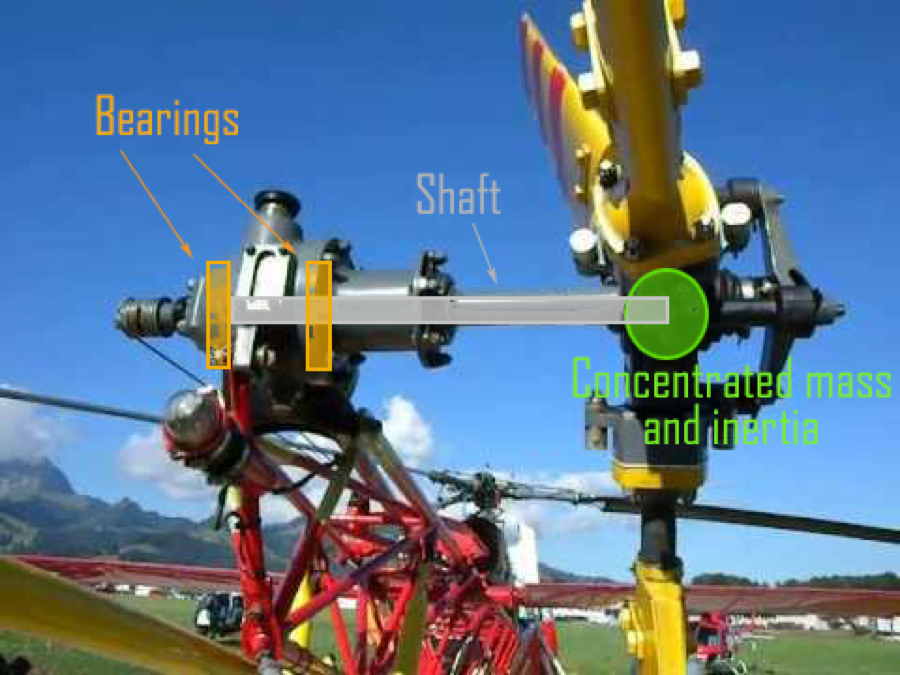
\includegraphics[width=.45\textwidth]{PICTURES/2_Lama_truss/PNG/model2/hqdefault2}} \quad
	\subfloat[][\emph{analysis model}.]
	{\includegraphics[width=.45\textwidth]{PICTURES/5_Rotordynamics/scheme.png}}\\
	\caption{Schemes of tail rotor assembly's model}
\end{figure}
%\vspace{0.5cm}

\subsection*{Model assumptions}
\addcontentsline{toc}{subsection}{Model assumptions}
\begin{itemize}
	\item Axial-symmetric structure (rotor-dynamics requirement in Ansys);
	\item Linear elastic material properties;
	\item Rotor elastically supported (2 bearings);
	\item Aerodynamic loads not considered;
	\item Rigid rotor and connections (no hinges or flexible joints).
\end{itemize}



\subsection*{Applied boundary conditions}
\addcontentsline{toc}{subsection}{Applied boundary conditions}
\noindent
\begin{itemize}
	\item Only fixed constraints are allowed for rotor-dynamic analysis;
	\item Support elasticity modelled using COMBIN14 elements to represent bearings;
\end{itemize}

\noindent
\textbf{COMBIN14} \\
Bearings have been modelled with COMBIN14 element whose properties simulate the effect of a longitudinal spring-damper as a axial tension-compression element.
The element is created between two nodes which, in our case, are overlapped. One of the nodes is rigidly attached to the shaft while the other one is constrained on the ground. These elements allows the elastic movement of the shaft in the Y and Z directions. The bearing is composed by 7 balls that ensure an overall stiffness equal to $378e+7$ N/m.\\

\medskip
\begin{figure}[h]
	\begin{center}
		\centering  		 		
		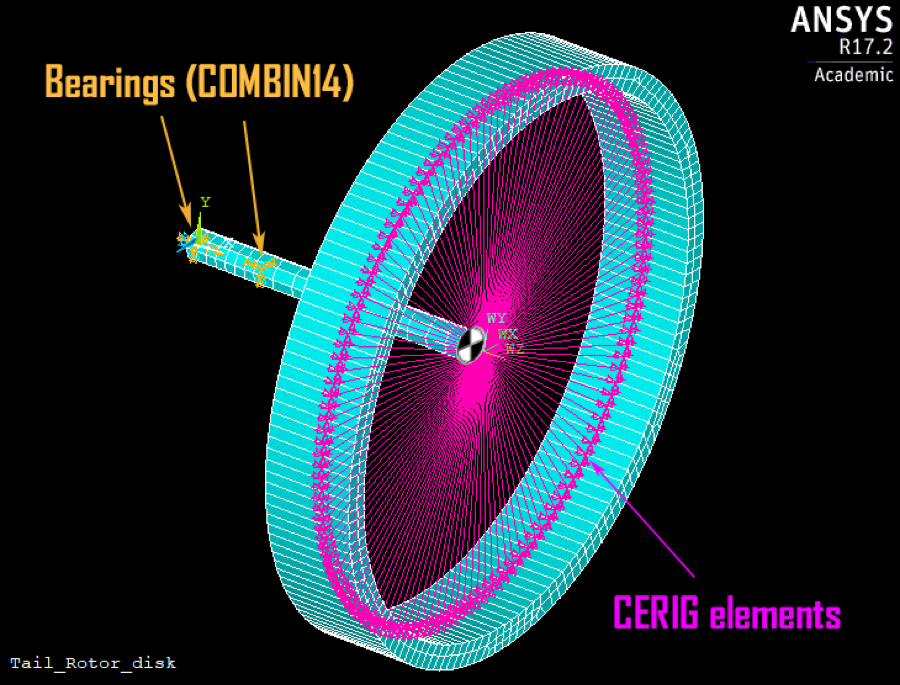
\includegraphics[width=0.55\linewidth]{PICTURES/5_Rotordynamics/2.png}
	\end{center}
	\caption {Tail rotor simplified model}
\end{figure}
%\vspace{0.5cm}

\clearpage
\subsection*{Solution including rotational effects (centrifugal and Coriolis)}
\addcontentsline{toc}{subsection}{Solution including rotational effects (centrifugal and Coriolis)}
\noindent
The modal analysis must be solved using an algorithm for damped modal analysis (complex Eigenvalues and Eigenvectors). We have chosen the \textbf{QRDAMP} solver including the rotational effects (\textbf{CORIOLIS, ON, , , ON}), as reported in listing (\ref{list:SolutionChunk}). The rotation speed (2000 RPM) has been divided in several load-steps. 10 modes have been extracted from each step. 

\lstinputlisting[firstline=133, lastline=146, language=apdl-modified,label={list:SolutionChunk}, caption=solution including rotational effects]{./COMMAND_LISTS/SOLO_ROTOR.txt}

\subsection*{Postprocessing}
\addcontentsline{toc}{subsection}{Postprocessing}
\noindent
Rotor's natural frequencies have been calculated for each value of the rotation speed (hence for each load step) and assigned to a substep. Resulting natural frequencies vary with the rotor speed as it is displayed in the campbell diagram below. \\
A \textbf{critical speed} appears when the natural frequency is equal to the excitation frequency, and excitation may come from unbalance that is synchronous with the rotational velocity. \\
Critical speeds are directly determined by solving a new eigenvalue problem or by performing a Campbell diagram analysis, where the intersection points between the frequency curves and the excitation line are calculated.

\noindent
The rotational velocity of the rotor is specified via the \textbf{CMOMEGA} command which requires to specify which is the rotating component, previously defined and selected as input for the velocity vector (magnitude and direction). \\
Then, we can set the \textbf{CAMPBELL, ON} Ansys' command. \\

\noindent
\textbf{NOTE:} \\
Bearing stiffness has an important effect on the critical speeds. When analysing a rotor, it is important to understand the effect of the bearing stiffness on the critical speeds and this can be done drawing the "Critical Speed Map" (here neglected).

\vspace{5mm}
\noindent
The rotor has been achieved with some parameters determined after performed a static analysis on ANSYS. The resulting given matrix provide us the information needed for establish some following conclusions:

\begin{equation*}
\left[ I \right] = \begin{bmatrix} 8.6440 & 0.1476 \times 10^{-3} & -0.3815 \times 10^{-4} \\ 0.1476 \times 10^{-3} & 14.487 & -0.1114 \times 10^{-3} \\ -0.3815 \times 10^{-4} & -0.1114 \times 10^{-3} & 13.895
\end{bmatrix} \quad
\end{equation*}

\vspace{3mm}
\noindent
As can be seen from the preceding matrix [\textit{I}], the diagonal guys refers to polar ($I_{p1}$ = 8.6440 $kg*m^2$) and diametrical inertia ($I_{d2}$ = 14.487 $kg*m^2$, $I_{d3}$ = 13.895 $kg*m^2$), respectively. From the literature, we expected 4 critical speeds, thanks to the fact that $I_{d}$ > $I_{p}$ for thick disc.
The results match with our expectation as we can notice from the Campbell plot below: 

\medskip
\begin{figure}[h]
	\begin{center}
		\centering  		 		
		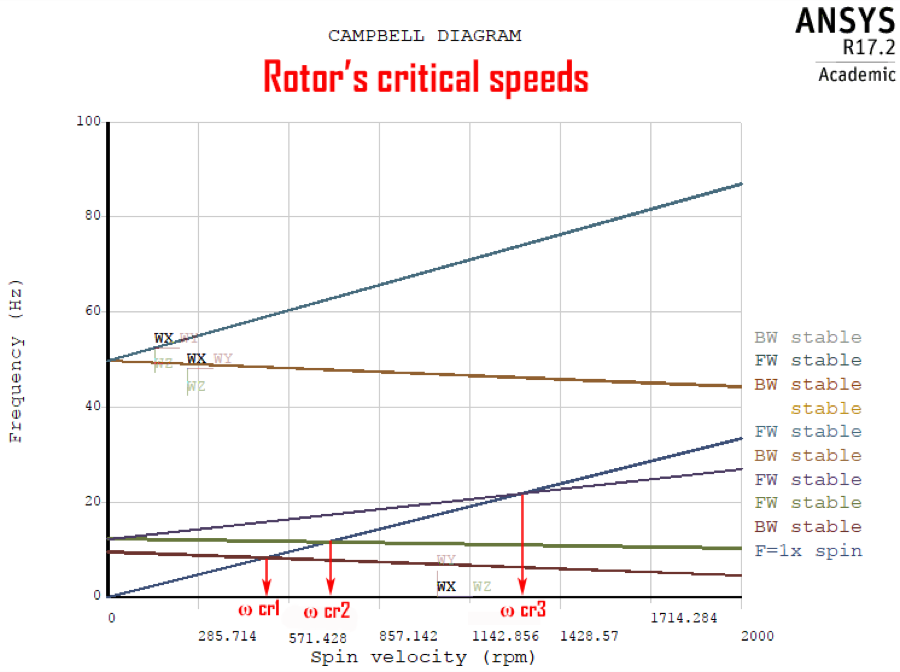
\includegraphics[width=1\linewidth]{PICTURES/5_Rotordynamics/campbell1.png}
	\end{center}
	\caption{Campbell diagram}
	\label{fig:critical speed} 
\end{figure}
%\vspace{0.5cm}

\begin{table}[h!]
	\centering
	\pgfplotstableset{
		% global config, for example in the preamble
		% these columns/<colname>/.style={<options>} things define a style
		% which applies to <colname> only.
		every head row/.style={before row=\hline,after row=\hline},
		every last row/.style={after row=\hline},
		display columns/0/.style={column name =Num, int detect,column type=r},
		display columns/1/.style={column name =Critical Speed [rpm], column type=r,
			fixed,fixed zerofill,precision=5,set thousands separator={\,}},
		%other style option   
	}
	\pgfplotstabletypeset[col sep=space]{VelocCritic-ModalAnalisys.txt}
	\caption{Natural frequencies for the simple model}
	\label{tab:ModalFreq-Shellmodel}
\end{table}
%
\noindent The fourth critical speed isn't shown in the figure~\ref{fig:critical speed} because is much higher than the full scale (2000 rpm), which value representing the nominal rotational speed of the rotor. We can even say that, with these results, it would be not advisable to design a rotor which is expected to operate at a velocity that stands in the middle of 2 of its critical speeds, since this range is typically UNSTABLE and inside it the onset of self-excited vibration phenomenon cannot be prevented.\\
However, this model does not represent the real tail rotor but it is just a very simplified model with the idea of explore the Ansys rotordynamics capabilities.\\
Hence, we can conclude that this value of speed appears unsafe from a dynamical point of view. In these cases, in order to be a rigid rotor, the literature suggests to change the geometrical parameters of the rotors, e.g. by adding or subtracting suitable masses or essentially \underline{by made torsionally stiffer the rotor shaft}. The idea of increase the stiffness of the shaft, from our point of view, could be a smart solution to solve this issue. Anyway, we are completely aware of the roughly results and so we can go on with the remaining analysis. One brief and further consideration is given relative to the resulting orbit motion of the rotor (whirling), that turns out by the gravitational static imbalance affecting the rotor structure and produces rotating bending of the shaft.

\medskip
\begin{figure}[h]
	\begin{center}
		\centering  		 		
		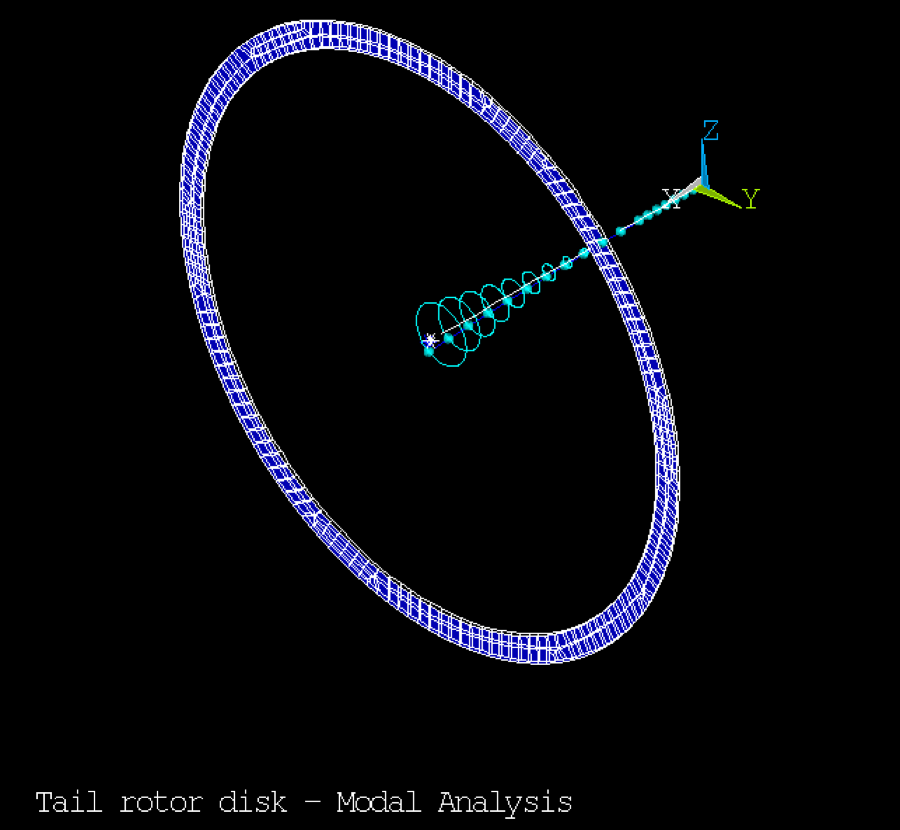
\includegraphics[width=0.45\linewidth]{PICTURES/5_Rotordynamics/ModalAnalisys004.png} 
	\end{center}
	\caption{Orbital motion of the rotor shaft}
\end{figure}

\subsection*{Coupling analysis}
\addcontentsline{toc}{subsection}{Coupling analysis}
\noindent Once realized the rotor, one attempt was given on mounting that system upon the main structure, in order to verify the rotor-tailboom coupling, starting with the hints written on the chapter~\ref{ch:Rotor-fuselage dynamic coupling}. Here, one goal is to check the vibrations exerted by the gravitational static imbalance of the rotor on the tailboom main structure and spend some words regarding modal shape and natural frequencies of the overall assembly. 

\medskip
\begin{figure}[h]	
	\centering
	\subfloat[][Truss model]  		 		
	{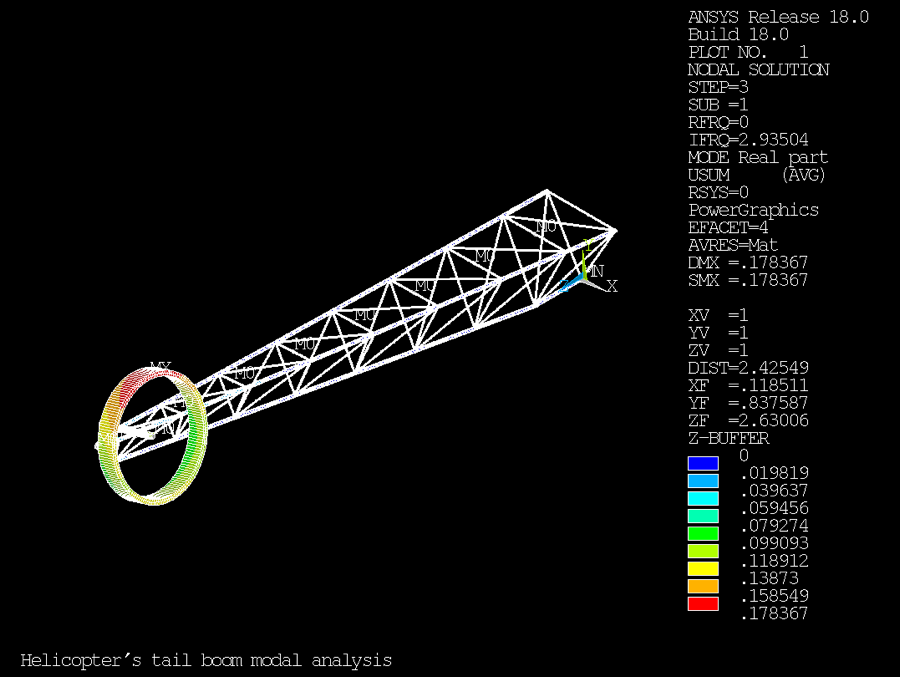
\includegraphics[width=0.45\linewidth]{PICTURES/5_Rotordynamics/TrussTailLumpedRotorRun003.png}} \quad
	\subfloat[][Shell model]
	{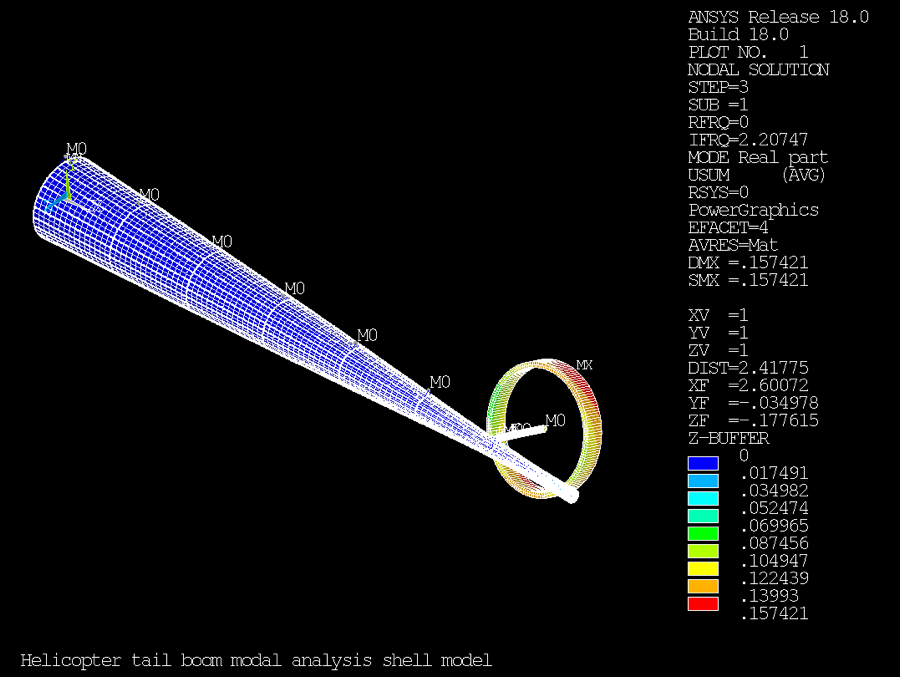
\includegraphics[width=0.45\linewidth]{PICTURES/5_Rotordynamics/ShellmodelShaftLumped005.png}} 
	\caption{Rotor - fuselage coupling}
	\label{Rotor - fuselage coupling}
\end{figure}

\noindent
Unfortunately, rotordynamics in ANSYS has no advanced tools to study asymmetric structures and, as we mentioned before, it performs and solve frameworks that are only axisymmetric respect to one principal axis. Indeed, we tried to follow this way, but ANSYS provide only information relative to the sole rotor (as we can observe from the figure~\ref{Rotor - fuselage coupling}), without take into account the coupling effect. This software lack pushed ourselves to don't proceed the analysis forward, even though could be a future matter of investigation.
